
%%%%%%%%%%%%%%%%%%%%%%% file typeinst.tex %%%%%%%%%%%%%%%%%%%%%%%%%
%
% This is the LaTeX source for the instructions to authors using
% the LaTeX document class 'llncs.cls' for contributions to
% the Lecture Notes in Computer Sciences series.
% http://www.springer.com/lncs       Springer Heidelberg 2006/05/04
%
% It may be used as a template for your own input - copy it
% to a new file with a new name and use it as the basis
% for your article.
%
% NB: the document class 'llncs' has its own and detailed documentation, see
% ftp://ftp.springer.de/data/pubftp/pub/tex/latex/llncs/latex2e/llncsdoc.pdf
%
%%%%%%%%%%%%%%%%%%%%%%%%%%%%%%%%%%%%%%%%%%%%%%%%%%%%%%%%%%%%%%%%%%%


\documentclass[runningheads,a4paper]{llncs}
%\documentclass[spanish]{llncs}

\usepackage{amssymb}
\setcounter{tocdepth}{3}
\usepackage{graphicx}
%\usepackage[spanish]{babel}
%\selectlanguage{spanish}
\usepackage[utf8]{inputenc}

\usepackage{url}
\urldef{\mailsa}\path|{kevin.ortiz, jhan.sierra, brayan.torres, 	christopher.vargas,|
	\urldef{\mailsb}\path|walter.arboleda, raquel.anaya}@unac.edu.co|
%	\urldef{\mailsc}\path ivan.paez@adlinktech.com
	\urldef{\mailsc}\path|ivan.paez@adlinktech.com|

\newcommand{\keywords}[1]{\par\addvspace\baselineskip
	\noindent\keywordname\enspace\ignorespaces#1}

\begin{document}
	
	\mainmatter  % start of an individual contribution
	
	% first the title is needed
	\title{Diagnóstico y Seguimiento de	Estilo de Vida Usando Internet de las Cosas}
	
	% a short form should be given in case it is too long for the running head
	\titlerunning{}
	
	% the name(s) of the author(s) follow(s) next
	%
	% NB: Chinese authors should write their first names(s) in front of
	% their surnames. This ensures that the names appear correctly in
	% the running heads and the author index.
	%
	\author{Kevin Ortiz
		\and Jhan Sierra \and Brayan Torres\and Christopher Vargas\and\\
		Walter Arboleda\and Raquel Anaya\and Ivan Paez}
	%
	\authorrunning{}
	% (feature abused for this document to repeat the title also on left hand pages)
	
	% the affiliations are given next; don't give your e-mail address
	% unless you accept that it will be published
	\institute{Corporacion Universitaria Adventista, UNAC,  Colombia\\
		\mailsa\\
		\mailsb\\
		\mailsc\\
		\url{}}
	
	%
	% NB: a more complex sample for affiliations and the mapping to the
	% corresponding authors can be found in the file "llncs.dem"
	% (search for the string "\mainmatter" where a contribution starts).
	% "llncs.dem" accompanies the document class "llncs.cls".
	%
	
	\toctitle{Lecture Notes in Computer Science}
	\tocauthor{Authors' Instructions}
	\maketitle
	
\begin{abstract}
Los grandes avances tecnológicos que son impulsados por la movilidad, los dispositivos inteligentes y el manejo de grandes volúmenes de datos, transforman las diversas áreas de actuación de la sociedad y del individuo, entre las que se encuentra la promoción de la salud. La actividad física y el descanso son dos aspectos centrales en la promoción de un estilo de vida saludable; la actividad física debe ser realizada considerando las características particulares del individuo y las condiciones del adecuadas del medio ambiente, tales como la contaminación del aire, que hoy en día representa una de las problemáticas de las grandes ciudades.
\end{abstract}


\section{Introducción}

Hace pocos meses, los países de la OCDE \footnote{The Organisation for Economic Co-operation and Development. \url{http://www.oecd.org/}} acordaron invitar a Colombia a convertirse en miembro de esta organización. En el marco de esta organizacion, el informe de Noviembre 2017 "¿Cómo va la vida en Colombia?" muestra el bienestar promedio en Colombia durante los últimos 10 años apartir de diferentes dimensiones, por ejemplo: ingresos y patrimonio financiero, empleo y remuneración, Vivienda, salud, educacion, entre otros \cite{vida_colombia}. En este articulo nos interesa contribuir nuestro grano de arena realizando un entudio enmarcado en la dimension del Medio ambiente, que nos permite contribuir al estudio de  los niveles de contaminación atmosférica en la ciudad de Medellin. 


\subsection{Objetivos}
Desarrollar una solución tecnológica para promover y monitorear la actividad física en una comunidad universitaria, teniendo en cuenta las condiciones biológicas del individuo y el nivel de contaminación del aire \cite{url_siata}.

\subsection{Metodo}

%\begin{tabular}{2}
	Fase 1 - Caracterización de la arquitectura para una solución integrada de movilidad con elementos de IoT
	
	
	
%\end{tabular}



\section{Arquitectura del Sistema}

La arquitectura del sistema esta descrita en la siguiente Figura \ref{fig:arquitectura}.

\begin{figure}
	\centering
	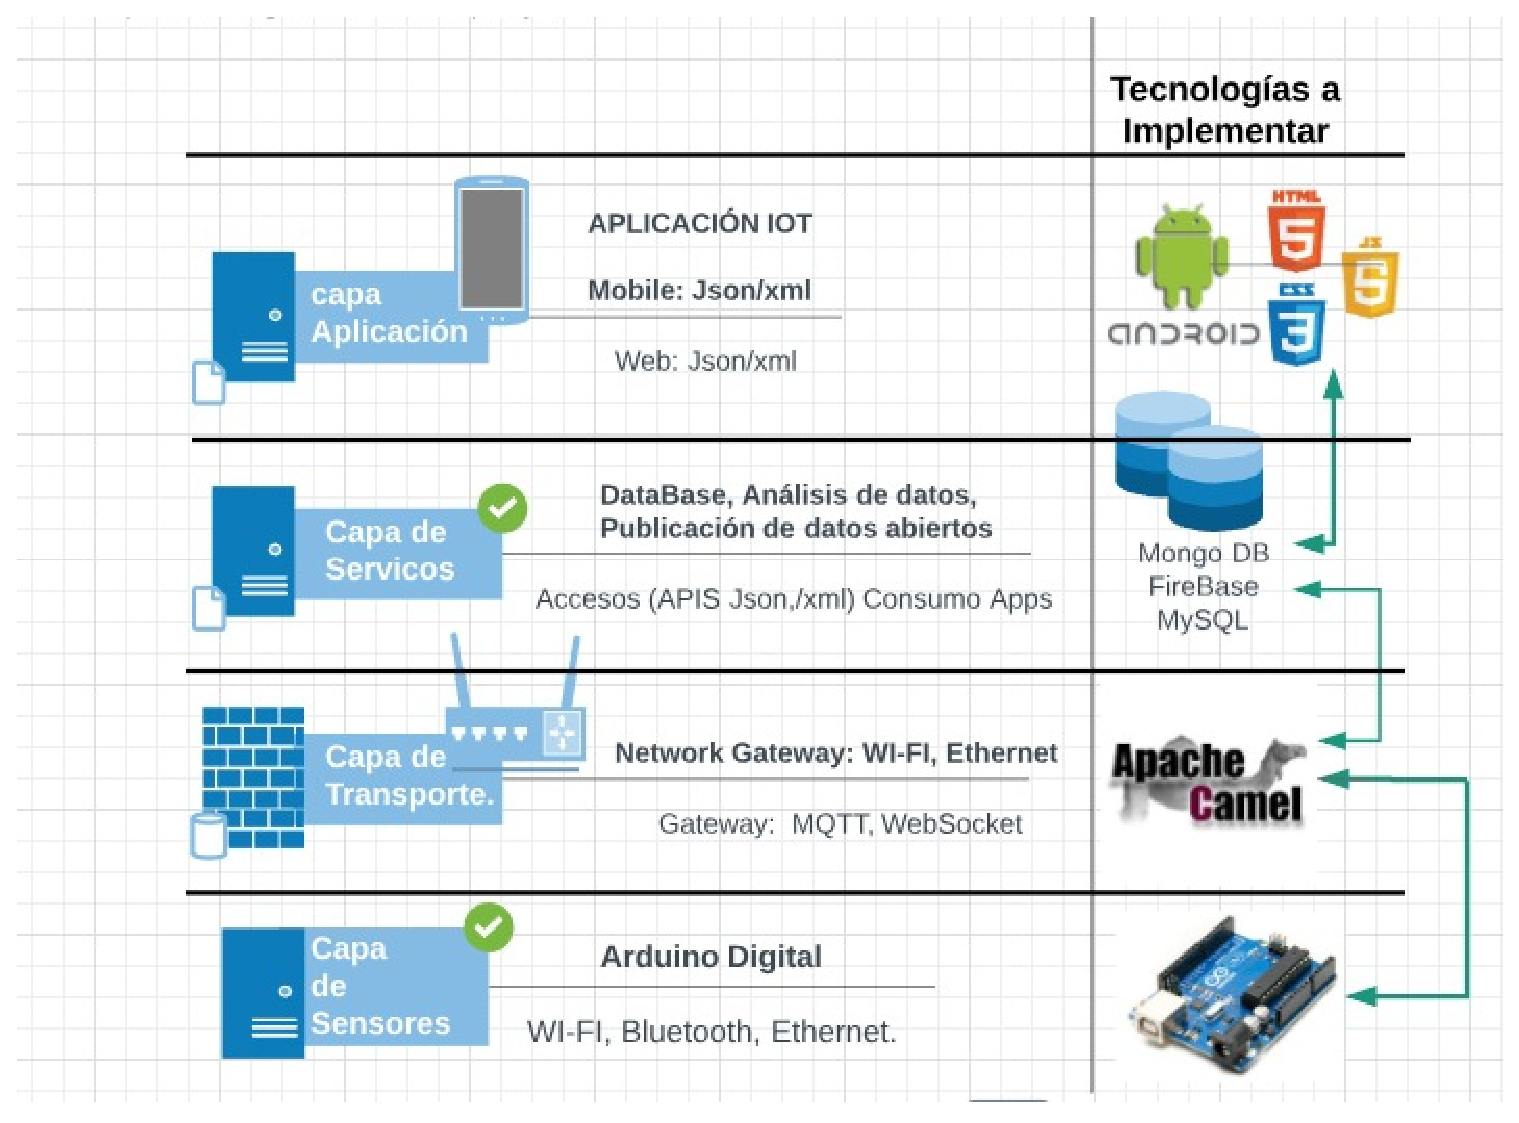
\includegraphics[height=8.2cm]{arquitectura2}
	\caption{Arquitectura del Sistema IoT}
	\label{fig:arquitectura}
\end{figure}

\section{Resultados}

Estudio y comprensión de Arquitectura IoT.
Selección de tecnologías y prueba de concepto de las capas de la arquitectura IoT.
Creación del ambiente de trabajo para implementación de la solución
Indagación  de sensores en el mercado para medir contaminación del aire y exploración  de manillas Wearable para monitorear descanso y actividad física \cite{proceeding1}\textsl{}.

\section{Conclusion}

Se ha obtenido conocimiento sustancial, en tecnología IoT, como también en la arquitectura de trabajo conjunto de sensores y plataformas de desarrollo


%\section{Referencias}\label{references}


\begin{thebibliography}{4}

\bibitem{vida_colombia}¿Cómo va la vida en Colombia?. Informe OCDE Noviembre 2017.
\url{http://www.oecd.org/countries/colombia/Better-Life-Initiative-country-note-Colombia-in-Espagnol.pdf}

\bibitem{proceeding1} R. Alley and A. Inc. Manual de Control de la Calidad del Aire,” in Calidad de Aire en America Latina, pp. 2–5. (2009)

\bibitem{url_siata} SIATA, “Sistema de alerta temprana del Area Metropolitana del Valle de Aburra”. \url{https://siata.gov.co/siata_nuevo/}



\end{thebibliography}

\end{document}
